\subsection{Example}

Let we introduce the next example. Grammar $G_1$ is a query and we want to find all paths in graph $M$ (presented in picture~\ref{input}) matched this query.
Result SPPF for this input is presented in picture~\ref{SPPF}. Note that presented version does not contains obsolete nodes.
Each terminal node corresponds with edge in the input graph: for each node with label $(v_0, T, v_1)$ there is $e\in E: e=(v_0,T,v_1)$.
We duplicate terminal nodes only for figure simplification.

\begin{figure}[h]
    \begin{center}
        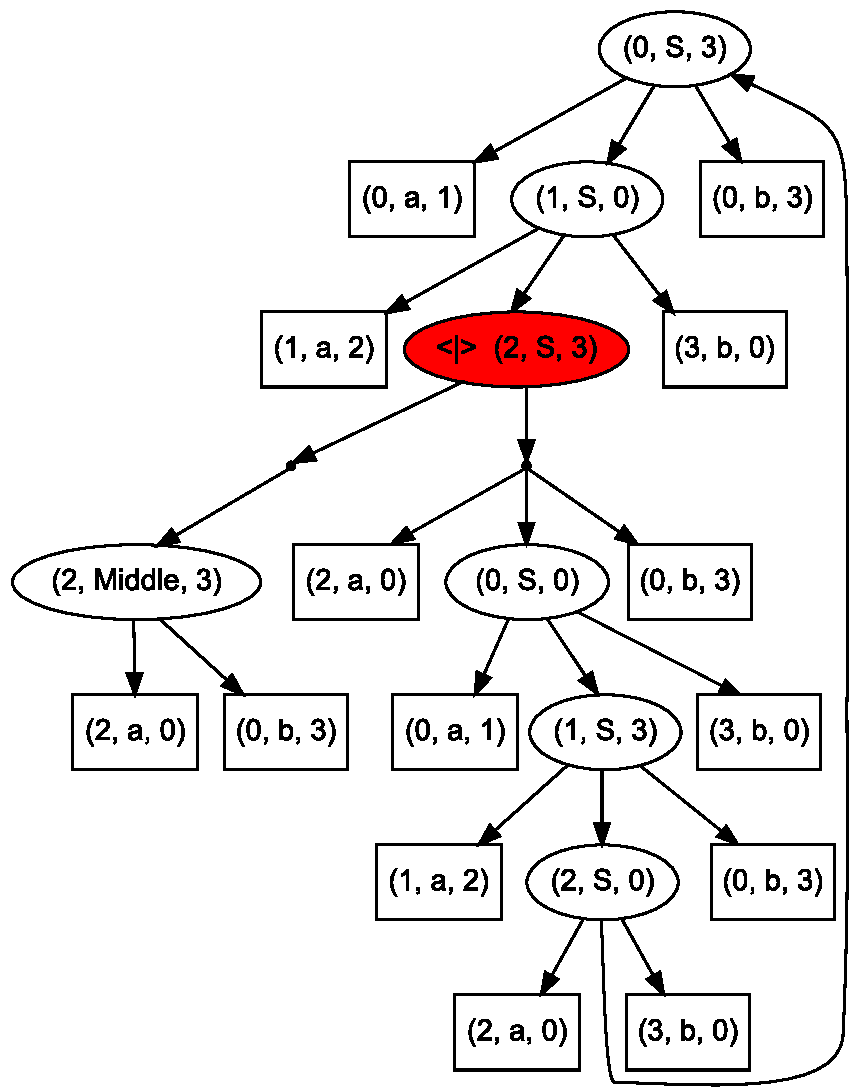
\includegraphics[width=8cm]{dot/AnBn.pdf}
        \caption{Result SPPF for input graph $M$(pic.~\ref{input}) and query $G_1$(pic.~\ref{grammarG})}
        \label{SPPF}        
    \end{center}
\end{figure}

	
As an example of derivation structure usage we can find 'middle' of any path in example above simply by finding corresponded nonterminal $middle$ in SPPF.
So we can found that there is only one common ancestor for all results, and it is vertex with $id = 0$. 

Extensions stored in nodes allow to check whether path from $u$ to $v$ exists, and extract it. 
To extract specified path we need only traverse SPPF, and it can be done in linear time (in terms of SPPF size). 

Let for example we want to find paths satisfying specified in $G_1$ constraints from vertex $0$.
To do this we should find vertices with label $(0, s, \_)$ in SPPF.
We can see that there are two vertices with required label: $(0, s, 0)$ and $(0, s, 3)$.
Next step let we try to extract corresponded paths from SPPF.
In our example there is cycle in SPPF so there are \textbf{at least} two different paths: $$p_0=\{(0,A,1);(1,A,2);(2,A,0);(0,B,3);(3,B,0);(0,B,3)\}$$ and 
\begin{align*}
p_1=\{&(0,A,1);(1,A,2);(2,A,0);(0,A,1);(1,A,2);(2,A,0);\\ &(0,B,3);(3,B,0);(0,B,3);(3,B,0);(0,B,3);(3,B,0)\}.
\end{align*}


Thus SPPF which constructed by described algorithm can be useful for query result investigation. 
But in some cases explicit representation of matched subgraph may be preferred, and required subgraph may be extracted from SPPF trivially by its traversal.
